\documentclass[a4paper, 11pt]{article}
\usepackage{cite,graphicx,amssymb,amsmath,amsthm,
enumerate,url,hyperref, cmap} 
\usepackage[numbers]{natbib}
\bibliographystyle{plainnat}

\newtheorem{theorem}{Theorem}
\newtheorem{lemma}{Lemma}
\newtheorem{definition}{Definition}
\newtheorem{proposition}{Proposition}

\title{Quaternions and Three-Dimensional Rotations}
\author{5601754}
\begin{document}
\date{}
\maketitle

\section{Introduction}
We first encountered quaternions in the Algebra 3 lecture notes where they were introduced as the group \(Q_8\), with the following presentation, 

    \[Q_8 = \langle a, b\ \mid \ a^4 = 1,\ a^2 = b^2,\ bab^{-1} = a^{-1} \rangle. \]
    
Upon researching this group, it is, in fact, a representation of Hamilton's famous extension of the complex plane, where the eight elements of the group are $\{\pm 1,\ \pm i, \ \pm j, \ \pm k\}$ and the multiplication formulae are those that William Rowan Hamilton carved into the stone of Broomebridge in Dublin \citep[p.~41]{lewis_2006_quaternion}. Now immortalised there by a plaque, these formulae are,

\[i^2 = j^2 = k^2 = ijk = -1.\]

Motivated by the potential uses of these imaginary numbers and their application in a very-much-not imaginary world; in this essay we will consider the vector representation of quaternions with their corresponding algebra, investigate how conjugating these four-dimensional numbers can represent rotations on a three-dimensional plane, and finally build increasingly more accurate methods of interpolating the rotations.

\section{Algebraic preliminaries for quaternions}

We denote the ring of quaternions as $\mathbb{H}$. Before we can confidently work with them, we need to define a representation, multiplication, addition, and other functions they have.

\par
\subsection{Representing a quaternion}
For any element \(p \in \mathbb{H}\) we can represent it as the following, 

\[p =  p_0 + p_1\boldsymbol{i} + p_2\boldsymbol{j} + p_3\boldsymbol{k} \quad \quad p_i \in \mathbb{R} , \ i \in \{ 0,1,2,3 \}.\]

We refer to the vector part of \(p\) as \(\boldsymbol{p} =(p_1,p_2,p_3) \in \mathbb{R}^3\). \citep[p.~2]{jia_2013_quaternions}



\subsection{Quaternion multiplication}
We can write quaternion multiplication in terms of the inner and cross products of the vector parts, for any \(p,q \in \mathbb{H}\), \citep[p.~2]{jia_2013_quaternions}

\[
\begin{aligned}
pq &= p_0 q_0 - \boldsymbol{p} \cdot \boldsymbol{q}
+ p_0 \boldsymbol{q}
+ q_0 \boldsymbol{p}
+ \boldsymbol{p}  \times \boldsymbol{q}.
\end{aligned}
\]


\subsection{Quaternion addition}

Quaternion addition is defined as the addition of a vector component-wise in $\mathbb{R}^4$. \citep[p.~2]{jia_2013_quaternions}

\subsection{Quaternion conjugate}

The complex conjugate of the quaternion 

\[p = p_0 \,+ \boldsymbol{p}\]

is denoted as

\[p^*= p_0 \,- \boldsymbol{p}.\] \citep[p.~3]{jia_2013_quaternions}

From this we obtain the following properties

\[
\begin{aligned}
(p^*)^* &=  p, \\[6pt]
p + p^* &= 2p_0, \\[6pt]
p^* p &= p p^* .
\end{aligned}
\] \citep[p.~3]{jia_2013_quaternions}

We also get the following proposition:

\begin{proposition}

    For any two $p,q \in \mathbb{H}$,

    \[(pq)^* = q^*p^*.\]
\end{proposition}
\begin{proof}

    This can be easily shown by expanding each side of the equation using the above definitions. 
\end{proof}


\subsection{Norm on quaternions}

The norm which we will use that acts on quaternions is represented as \(|p|\) and is defined as follows

\[|p| = \sqrt{p^*p}.\]

Since 
\[p^*p = p_0^2 + p_1^2 + p_2^2 + p_3^2,\]

it follows that the norm on quaternions is equivalent to the usual norm of $\mathbb{R}^4$, thus is a well-defined norm. The following proposition is used in the proof of a later lemma.

\begin{proposition}

    The quaternion norm is multiplicative.
\end{proposition}

\begin{proof}
    Consider

    \[|pq|^2 = (pq)(pq)^* = (pq)(q^*p^*) = p(qq^*)p^*,\]
    
    by associativity of quaternion multiplication \citep[p.~166]{dunn_parberry_2002}. We then obtain

    \[|pq|^2 = p|q|^2p^* = pp^*|q|^2 = |p|^2|q|^2.\]

    Square rooting provides $|pq| = |p||q|$, as required.

\end{proof}

Note that a quaternion with $|p|= 1$ is known as a unit quaternion. The subgroup of the multiplicative group of $\mathbb{H}$ that contains only unit quaternions will be denoted as $\mathbb{H}_1$.

\subsection{Quaternion inverse}

The inverse of a quaternion is denoted

\[p^{-1} = \frac{p^*}{|p|^2}.\] \citep[p.~3]{jia_2013_quaternions}

Note that if \(p\) is a unit quaternion, then \(p^{-1} = p^*\)

\subsection{Trigonometric representation of a unit quaternion}

Let us consider a unit quaternion $q=q_0 + \boldsymbol{q}$ then, 

\[1= |q|^2 = q^*q = q_0^2+ ||\boldsymbol{q}||^2.\]

This implies that there exists some angle $\theta$ such that 



\[
\begin{aligned}
\cos^2\theta &= q_0^2 \\
\sin^2\theta &= ||\boldsymbol{q}||^2.\\
\end{aligned}\]

Due to the periodicity of $\sin^2\theta$ and $\cos^2\theta$, there is a unique $\theta \in [0,\pi]$ such that $\cos\theta = q_0 $ and $\sin\theta = ||\boldsymbol{q}||$. Defining a unit vector $\boldsymbol{u} = \frac{\boldsymbol{q}}{||\boldsymbol{q}||} \in \mathbb{R}^3$, we can write a unit quaternion as

\[ q = \cos\theta + \boldsymbol{u}\sin\theta.\]
\citep[p.~4]{jia_2013_quaternions}

Note that in the context of 3-dimensional rotations, the quaternion angle $\theta$ corresponds to half the rotation when it is applied to a vector. This will be shown in Section 3. 
 
\subsection{Quaternion logarithm and exponential}

First, let us define a pure quaternion as a quaternion with a real part of $0$.

The logarithm of a unit quaternion $q$ is defined as

\[\log q = \log (\cos\theta  + \boldsymbol{u}\sin\theta) =   0 + \theta \boldsymbol{u}.\] \citep[p.~170]{dunn_parberry_2002}

The exponential of a  quaternion must take a pure quaternion, $p = 0 + \theta\boldsymbol{u}$ and is defined as 

\[\exp p = \exp (0 +\theta\boldsymbol{u}) = \cos \theta + \boldsymbol{u}\sin\theta.\] \citep[p.~170]{dunn_parberry_2002}

\subsection{Quaternion exponentiation}

Quaternion exponentiation is raising a quaternion to a scalar power. As the exponent varies from $0$ to $1$, the value of $q^t$ varies from $1 + \boldsymbol{0}$ to $q$. 

This allows us to take a fraction of the angular displacement. It is defined as

\[q^t = \exp(t \log  q).\]  \citep[p.~171]{dunn_parberry_2002}

The fraction of angular displacement is clear when we use the above definitions to expand the exponentiation to

\[q^t = \exp(t \log  q) = \exp(t (0+\theta\boldsymbol{u})) = \exp(0+t\theta\boldsymbol{u}) = \cos (t\theta) + \boldsymbol{u}\sin (t\theta).\] 

\section{Quaternion Rotation Theorem}

The Quaternion Rotation Theorem is based on the operator

\[L_q(\boldsymbol{v}) = q\boldsymbol{v}q^*.\]

Within the proof, we will need to make use of three lemmas. 

\begin{lemma}(Length Preservation)

    For any unit quaternion $q$, the operator \(L_q(\boldsymbol{v})\) preserves length.
\end{lemma}

\begin{proof} Using Proposition 2, the multiplicity of the norm on quaternions, 
    \[
        ||L_q(\boldsymbol{v})|| = |q\boldsymbol{v}q^*|
    = |q| \cdot ||\boldsymbol{v}|| \cdot |q^*| = ||\boldsymbol{v}|| \ \text{(since $|q| = 1$)}.\]
\end{proof}

\begin{lemma}(Parallel Invariance)

    If a vector $\boldsymbol{v}$ is parallel to the axis of rotation $u$ (the unit of the vector part of $q$), then it is invariant under $L_q(\boldsymbol{v})$.
\end{lemma}

\begin{proof}
    Let $\boldsymbol{v}$ = $k\boldsymbol{u}$ with $k \in \mathbb{R}$. Because $\boldsymbol{v}$ is parallel to the vector part of $q$, their cross product is $0$, so they commute under quaternion multiplication. Therefore

    \[L_q(\boldsymbol{v}) = q(k\boldsymbol{u})q^* = k\boldsymbol{u}(qq^*) = ku = \boldsymbol{v}.\]
\end{proof}

\begin{lemma}(Linearity of operator)

    The operator $L_q(\boldsymbol{v})$ is linear.
\end{lemma}

\begin{proof}

    \[L_q(a_1\boldsymbol{v}_1 + a_2\boldsymbol{v}_2) = q(a_1\boldsymbol{v}_1 + a_2\boldsymbol{v}_2)q^*.\]
    
    As quaternion multiplication is distributive (easily provable component-wise so shall not be proved here to stay concise)
    
    \[
        q(a_1\boldsymbol{v}_1 + a_2\boldsymbol{v}_2)q^*= q(a_1\boldsymbol{v}_1)q^* + q(a_2\boldsymbol{v}_2)q^*.
    \]
    
    Note that scalars commute with quaternion multiplication because they commute with both the inner product and the cross product. Thus
    
    \[
    q(a_1\boldsymbol{v}_1)q^* + q(a_2\boldsymbol{v}_2)q^* = a_1(q\boldsymbol{v}_1q^*) + a_2(q\boldsymbol{v}_2q^*) \\
    = a_1L_q(\boldsymbol{v}_1) + a_2L_q(\boldsymbol{v}_2).\]
    
\end{proof}


\begin{theorem}(Quaternion Rotation Theorem) \citep[p.~132]{kuipers_1999_quaternions}

For any unit quaternion

\[q = q_0 + \boldsymbol{q}= \cos\frac{\theta}{2} + \boldsymbol{u}\sin\frac{\theta}{2}\]

and for any vector $\boldsymbol{v} \in \mathbb{R}^3$, the action of the operator $L_q : \mathbb{R}^3 \to \mathbb{R}^3$ defined by 

\[L_q(\boldsymbol{v}) = q\boldsymbol{v}q^*\]

is equivalent to a rotation of the vector $\boldsymbol{v}$ through an angle $\theta$ about $\boldsymbol{u}$.

\end{theorem}

\begin{figure}[htbp]
    \centering
    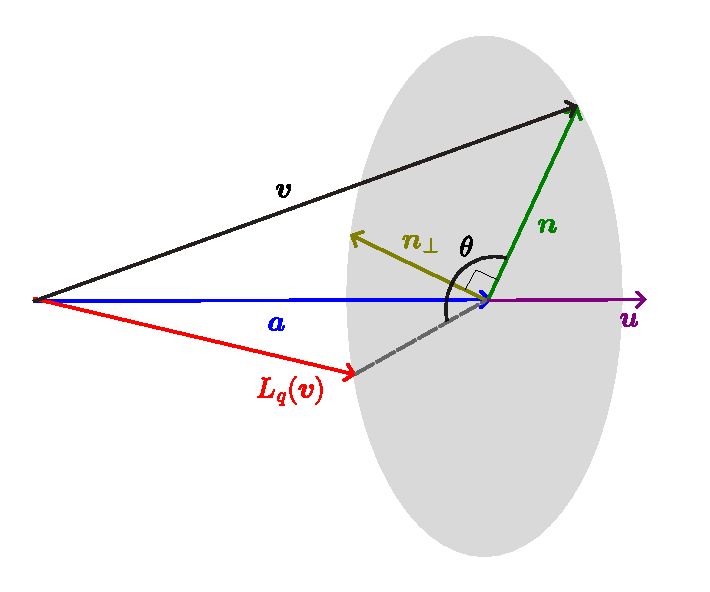
\includegraphics[width=0.8\textwidth]{QuaternionDiagram.pdf} 
    \caption{The decomposition into parallel and orthogonal components of a vector $\boldsymbol{v}$ rotated an angle of $\theta$ around $\boldsymbol{u}$. This image was the author's own work.}
    \label{fig:rotation_diag}
\end{figure}


\begin{proof}

Given $\boldsymbol{v} \in \mathbb{R}^3$, split it into two components, $\boldsymbol{v} = \boldsymbol{a} +\boldsymbol{n}$, where $\boldsymbol{a}$ is the component of the vector $\boldsymbol{v}$ which is parallel to  $\boldsymbol{u}$ and $\boldsymbol{n}$ as the component orthogonal to $\boldsymbol{u}$. Then to show that $L_q(\boldsymbol{v})$ functions as a rotation, we need to show that $\boldsymbol{a}$ is preserved and $\boldsymbol{n}$ is rotated about $\boldsymbol{u}$ at an angle of $\theta$. See Figure 1 for the geometric intuition for this.

By Lemma 3 (Linearity), $L_q(\boldsymbol{a} + \boldsymbol{n}) = L_q(\boldsymbol{a}) + L_q(\boldsymbol{n})$. By Lemma 2, $L_q(\boldsymbol{a}) = \boldsymbol{a}$.

 Focusing on the effect on the normal component $\boldsymbol{n}$ we have

\[L_q(\boldsymbol{n}) = q\boldsymbol{n}q^*.\]

First, let us consider 

\[q\boldsymbol{n} = -\boldsymbol{q} \cdot \boldsymbol{n}  +q_0\boldsymbol{n} + \boldsymbol{q} \times \boldsymbol{n}.\]

Note that $-\boldsymbol{q} \cdot \boldsymbol{n}$ is the scalar part of this quaternion and $q_0\boldsymbol{n} + \boldsymbol{q} \times \boldsymbol{n}$ is the vector part. Then

\[ \begin{aligned}
q\boldsymbol{n}q^* &= (-\boldsymbol{q} \cdot \boldsymbol{n}  +q_0\boldsymbol{n} + \boldsymbol{q} \times \boldsymbol{n})(q_0 - \boldsymbol{q})\\
&= (-\boldsymbol{q} \cdot \boldsymbol{n})q_0  - (q_0\boldsymbol{n} + \boldsymbol{q} \times \boldsymbol{n})\cdot (-\boldsymbol{q}) +(-\boldsymbol{q} \cdot \boldsymbol{n})(-\boldsymbol{q}) +q_0(q_0\boldsymbol{n} + \boldsymbol{q} \times \boldsymbol{n})\\ &+(q_0\boldsymbol{n}+ \boldsymbol{q} \times \boldsymbol{n}) \times (-\boldsymbol{q}).
\end{aligned}
\]

Expanding these brackets gives 

\[
\begin{aligned}L_q(\boldsymbol{n})&=-q_0(\boldsymbol{n}\cdot \boldsymbol{q}) +q_0(\boldsymbol{n}\cdot \boldsymbol{q})  -\boldsymbol{q} \cdot (\boldsymbol{q}\times\boldsymbol{n})+ \boldsymbol{q}(\boldsymbol{n} \cdot \boldsymbol{q})\\ &+ q_0^2 \boldsymbol{n} + q_0(\boldsymbol{q}\times \boldsymbol{n}) - q_0(\boldsymbol{n} \times \boldsymbol{q}) + (\boldsymbol{q} \times \boldsymbol{n} ) \times (-\boldsymbol{q}).\end{aligned}
\]

Using $(\boldsymbol{q}\times\boldsymbol{n}) = -(\boldsymbol{n} \times \boldsymbol{q})$, $(\boldsymbol{q} \times \boldsymbol{n}) \times (-\boldsymbol{q}) = -\boldsymbol{n}(\boldsymbol{q}\cdot \boldsymbol{q}) + \boldsymbol{q}(\boldsymbol{q}\cdot \boldsymbol{n})$ and $\boldsymbol{q}\cdot(\boldsymbol{q} \times \boldsymbol{n}) = 0$, we can reduce the equation to

\[\begin{aligned}
L_q(\boldsymbol{n})&= \boldsymbol{q}(\boldsymbol{n} \cdot \boldsymbol{q}) + q_0^2\boldsymbol{n} +2q_0(\boldsymbol{q} \times\boldsymbol{n}) -\boldsymbol{n}(\boldsymbol{q} \cdot \boldsymbol{q}) + \boldsymbol{q}(\boldsymbol{n} \cdot \boldsymbol{q})\\
&=\boldsymbol{n}(q_0^2-||\boldsymbol{q}||^2) + 2\boldsymbol{q}(\boldsymbol{n} \cdot \boldsymbol{q}) + 2q_0(\boldsymbol{q}\times\boldsymbol{n}).
\end{aligned}
\]

As $\boldsymbol{n}$ is orthogonal to $\boldsymbol{q}$, their dot product is zero, hence we get

\[\begin{aligned}
L_q(\boldsymbol{n}) &= \boldsymbol{n}(q_0^2-||q||^2)+2q_0(\boldsymbol{q}\times \boldsymbol{n})\\
&=\boldsymbol{n}(q_0^2-||q||^2) + 2q_0||\boldsymbol{q}||(\boldsymbol{u}\times\boldsymbol{n}),
\end{aligned}
\]
where $\boldsymbol{u} = \frac{\boldsymbol{q}}{||\boldsymbol{q}||}$. Let $\boldsymbol{n}_\perp = \boldsymbol{u} \times \boldsymbol{n}$. So,

\[L_q(\boldsymbol{n}) = \boldsymbol{n}(q_0^2-||q||^2)+2q_0||\boldsymbol{q}||\boldsymbol{n}_\perp.\]

We see that $\boldsymbol{n}_\perp$ and $\boldsymbol{n}$ have the same length,

\[||\boldsymbol{n}_\perp|| = ||(\boldsymbol{n} \times \boldsymbol{u})|| = ||\boldsymbol{n}|| \cdot ||\boldsymbol{u}|| \sin \frac{\pi}{2} = ||\boldsymbol{n}||.\]

Using our trigonometric identities from above, rewrite

\[
\begin{aligned}
L_q(\boldsymbol{n})
&=
\left(\cos^2 \frac{\theta}{2} - \sin^2 \frac{\theta}{2}\right)\boldsymbol{n}
+
\left(2\cos \frac{\theta}{2}\sin \frac{\theta}{2}\right)\boldsymbol{n}_{\perp} \\
&= \cos\theta\,\boldsymbol{n} + \sin\theta\,\boldsymbol{n}_{\perp}.
\end{aligned}
\]
This is clearly a rotation of $\boldsymbol{n}$ through an angle $\theta$ in the plane defined by $\boldsymbol{n}$ and $\boldsymbol{n}_\perp$, which is orthogonal to the rotation axis.


\end{proof}

\section{Applying quaternion rotations}

Now, let us say that we have a robotic arm that we want to move smoothly through three-dimensional space. Our rotator operator applies a quaternion to rotate a three-dimensional vector; now we just need a series of quaternions to operate on to smoothly transform from a starting orientation to an ending one (whilst maintaining a constant angular velocity). This means we need to interpolate from a starting quaternion to a final one.

This is not a trivial task. We cannot linearly interpolate because that would move from one quaternion to another following the shortest linear path, consequently, the length of the quaternion drops below one, stopping it being a unit quaternion. This invalidates Lemma 1, so we can no longer apply the rotator operator. This means we have to keep the quaternion length at one, i.e. move between quaternions by "walking" over the surface of a four-dimensional sphere. This leads to a process called Spherical linear interpolation (Slerp). \citep[p.~248]{shoemake_1985}

\subsection{Spherical linear interpolation (Slerp)}

We need a function \[Slerp(p,q,t): \mathbb{H}_1 \times \mathbb{H}_1 \times [0,1] \curvearrowright \mathbb{H}_1.\]

To construct this, we need a map which takes $p$ to $q$, trivially this is $p^{-1}q$, and then we want to take a fraction of this map over time. Recall from the definition of quaternion exponentiation in Section 2.9, we can consider raising it to the power of a $t$ between zero and one to interpolate the rotational angle. So let us try

\[Slerp(p,q,t) =p(p^{-1}q)^t\] \citep[p.~43]{dam_koch_lillholm_1998}

For this to be our desired function, we need to check that this has constant angular velocity. First, we need a proposition on differentiating quaternions. 

\begin{proposition}
    Let $q = \cos\theta + \boldsymbol{u}\sin\theta  \in \mathbb{H}_1 , t\in \mathbb{R}$. Then

    \[\frac{d}{dt} q^t = q^t\log(q).\] \citep[p.~23]{dam_koch_lillholm_1998}
\end{proposition}
\begin{proof}

    This is shown by calculating the derivative then selectively expanding the equation to rewrite it in an exponential form. 

    \begin{align*}
    \frac{d}{dt} q^t &=\frac{d}{dt}\exp(t\log(q))=\frac{d}{dt}\exp(t(0+\theta\boldsymbol{u}))\\&=\frac{d}{dt}(\cos (t \theta) + \sin (t\theta) \boldsymbol{u}) = -\theta\sin(t\theta) + \theta\cos(t\theta)\boldsymbol{u} \\ &=-\theta\sin(t\theta)(\boldsymbol{u}\cdot\boldsymbol{u})+\theta\cos(t\theta)\boldsymbol{u} + \theta\sin(t\theta)(\boldsymbol{u}\times\boldsymbol{u}) \\&= (\cos(t\theta) + \sin(t\theta)\boldsymbol{u})(0+\theta\boldsymbol{u}) \\&= \exp(t\log(q))\log(q) \\&= q^t\log(q).\end{align*}
    
\end{proof}

\begin{lemma}(Angular velocity)

The position vector function of $Slerp(p,q,t)$ has constant angular velocity \cite[pp.~45--46]{dam_koch_lillholm_1998}
\end{lemma}

\begin{proof}

Recall that our interpolation is restricted to the surface of a four-dimensional hypersphere. To prove the lemma, we need to show that its tangential acceleration is zero, or alternatively that the total acceleration vector points strictly towards the origin of the circle, directly opposing the position vector, mathematically we can write this as:

\[\frac{\partial^2}{\partial t^2}Slerp(p,q,t)   =c\cdot Slerp(p, q, t) \quad \text{where} \quad c \le 0.\]

To show that this is true, using Proposition 3 we find the following 

\begin{align*}\frac{\partial}{\partial t}Slerp(p,q,t) &= \frac{\partial}{\partial t} p(p^{-1}q)^t\\ &= p(p^{-1}q)^t\log (p^{-1}q) \\  &= Slerp(p,q,t)\log(p^{-1}q).\end{align*} 

\begin{align*}\frac{\partial^2}{\partial t^2}Slerp(p,q,t) &=  p(p^{-1}q)^t\log (p^{-1}q)^2 \\  &= Slerp(p,q,t)\log(p^{-1}q)^2\end{align*}

It is left to show that $\log(p^{-1}q)^2$ exists and is a non-positive real number. As $p^{-1},q \in \mathbb{H}_1$ then $p^{-1}q \in \mathbb{H}_1$, so there exists $\theta \in \mathbb{R}, \boldsymbol{u} \in \mathbb{R}^3$ such that $p^{-1}q = \cos\theta + \boldsymbol{u}\sin\theta$. This means

\[\log(p^{-1}q)^2 = (0 +\theta\boldsymbol{u})^2 = -\theta^2 (\boldsymbol{u}\cdot \boldsymbol{u}) + \boldsymbol{u} \times \boldsymbol{u} = -\theta^2.\]

Thus, $\frac{\partial^2}{\partial t^2}Slerp(p,q,t)   =c\cdot Slerp(p, q, t) \quad \text{where} \quad c = -\theta^2 \le 0$.
\end{proof}

We have found our desired Slerp function, which we can apply in conjunction with our rotation theorem to program a robotic arm, for example, to move at constant velocity between two points in three-dimensional space. However, a robotic arm would not just move between point A and point B, it would be following a chain of points, and whilst velocity is constant between two adjacent points, it is not necessarily constant throughout this chain. Let us try to find a new function that includes this.

\subsection{Spherical Splines (Squad)}

To eliminate this instantaneous change in velocity, which a robotic arm would not be able to perform, we need a curve which goes through a selection of "control points" at a constant velocity. To do this, we must form a continuously differentiable curve which passes through each point. This gives us $Squad$, originally formulated by Shoemake but referenced in \citet[p.~51]{dam_koch_lillholm_1998}.

\begin{definition}(Squad function)
\[Squad(q_i,q_{i+1},s_i,s_{i+1},t) = Slerp(Slerp(q_i,q_{i+1},t),Slerp(s_i,s_{i+1} ,t),2t(1-t)),\]

\[s_i = q_i \exp \left( -\frac{\log (q_i^{-1}q_{i+1}) + \log (q_i^{-1}q_{i-1})}{4} \right).\]

\end{definition}

With $t\in [0,1]$, an ordered series of unit control point quaternions $q_i \in \mathbb{H}_1 , i \in \{0,1, \dots , n \}$ and a 
series of corresponding tangential quaternions $s_i\in \mathbb{H}_1,  i \in \{0,1, \dots , n \} $. Notice that at the end points we are not able to create an $s_0$ or $s_n$, therefore certain boundary conditions, such as $s_0 = q_0, s_n =q_n$ need to be applied, depending on the real-world application.

Before proving that $Squad$ is a continuously differentiable function, we need a more advanced proposition on quaternion differentiation. 

\begin{proposition}

Let $q \in \mathcal{C}^1(\mathbb{R}, \mathbb{H}_1), r \in \mathcal{C}^1(\mathbb{R}, \mathbb{R})$. Since $q$ maps onto $\mathbb{H}_1$, $q(t)$ can be written as $\cos \theta(t) +  \boldsymbol{u}(t)\sin \theta (t) = \left[ \cos \theta(t),  \boldsymbol{u}(t)\sin \theta (t) \right]$ and we have

\begin{align*}
\frac{d}{d t} q(t)^{r(t)} &= \Bigl[ -\sin(r(t)\theta(t)) (r'(t)\theta(t) + r(t)\theta'(t)), \\
    &\quad \cos(r(t)\theta(t)) (r'(t)\theta(t) + r(t)\theta'(t)) \boldsymbol{u}(t) + \sin(r(t)\theta(t)) \boldsymbol{u}'(t) \Bigr]
\end{align*}

\citep[pp.~24--25]{dam_koch_lillholm_1998}

\end{proposition}

\begin{proof}

    \[
        q(t)^{r(t)} = [\cos(r(t)\theta(t),\boldsymbol{u}\sin(r(t)\theta(t)]
    \]

    Now let $\Theta(t) =r(t) \theta(t)$, then differentiating component-wise

    \begin{align*}
        &\frac{d}{dt}\cos(\Theta(t))  = -\sin(\Theta(t))\Theta'(t),\\&
        \frac{d}{dt}\boldsymbol{u}(t)\sin(\Theta(t) = \cos(\Theta(t))(t)\Theta'(t)\boldsymbol{u}(t) +\sin(\Theta(t))\boldsymbol{u}'(t), 
    \end{align*}

    using the product rule as shown by \citet[p.~24]{dam_koch_lillholm_1998}.

    Clearly $\Theta'(t) = r'(t)\theta(t) + r(t)\theta'(t)$, so substituting our values in gives

    \begin{align*}
        &[-\sin(\Theta(t))\Theta'(t),\cos(\Theta(t))(t)\Theta'(t)\boldsymbol{u}(t) +\sin(\Theta(t))\boldsymbol{u}'(t) ] = \\
        & \Bigl[ -\sin(r(t)\theta(t)) (r'(t)\theta(t) + r(t)\theta'(t)), \\
    &\quad \cos(r(t)\theta(t)) (r'(t)\theta(t) + r(t)\theta'(t)) \boldsymbol{u}(t) + \sin(r(t)\theta(t)) \boldsymbol{u}'(t) \Bigr].
    \end{align*}
\end{proof}

Now it is left to prove that $Squad$ is continuously differentiable. 
\begin{lemma}

    $Squad \in \mathcal{C}^1$      
    \citep[pp.~52--54]{dam_koch_lillholm_1998}
\end{lemma}

\begin{proof}

    It is clear that Squad is differentiable between each control point, as we have shown that Slerp has constant velocity between each point. Thus, we only need to consider continuous differentiability at a given control point $q_i$.

    First, we need to show that each adjacent segment has the same control point as their respective end and start, i.e. 
    \[Squad(q_{i-1},q_i,s_{i-1},s_i,1) = q_i = Squad(q_i,q_{i+1},s_i,s_{i+1},0).\]
    \begin{align*}
        Squad(q_{i-1},q_i,s_{i-1},s_i,1) &= Slerp(Slerp(q_{i-1},q_i,1),Slerp(s_{i-1},s_i,1),0) \\ &= Slerp(q_i,s_i,0) \\&= q_i.
    \end{align*}
    \begin{align*}
        Squad(q_i,q_{i+1},s_i,s_{i+1},0) &= Slerp(Slerp(q_i,q_{i+1},0),Slerp(s_i,s_{i+1} ,0),0) \\& = Slerp(q_i,s_i,0) \\&= q_i.
    \end{align*}

    Thus, $Squad$ is continuous and has the correct value at the control points. To show that it is continuously differentiable, we derive it in a given interval, then we show that these are equal as they meet at each control point, i.e 
    \[\frac{\partial}{\partial t}Squad(q_{i-1},q_i,s_{i-1},s_i,1) = \frac{\partial}{\partial t}Squad(q_i,q_{i+1},s_i,s_{i+1},0).\]

    We let
    \[g_i(t) = Slerp(q_i,q_{i+1},t)^*Slerp(s_i,s_{i+1} ,t).\]

    Now we find
    \begin{align*}
    \frac{\partial}{\partial t} Squad(q_i, q_{i+1}, s_i, s_{i+1}, t) &= \frac{\partial}{\partial t} Slerp(Slerp(q_i, q_{i+1}, t), Slerp(s_i, s_{i+1}, t), 2t(1-t)) \\
    &= \frac{\partial}{\partial t} \left(Slerp(q_i, q_{i+1}, t) g_i(t)^{2t(1-t)} \right).
    \end{align*}

    Then using the product rule,
    \begin{align*}
    \frac{\partial}{\partial t} Squad(q_i, q_{i+1}, s_i, s_{i+1}, t) &= \frac{\partial}{\partial t} \left( Slerp(q_i, q_{i+1}, t) g_i(t)^{2t(1-t)} \right) \\
    &= \left( \frac{\partial}{\partial t} (Slerp(q_i, q_{i+1}, t)) \right) g_i(t)^{2t(1-t)} + \\
    &\quad Slerp(q_i, q_{i+1}, t) \left( \frac{\partial}{\partial t} (g_i(t)^{2t(1-t)}) \right) \\
    &= Slerp(q_i, q_{i+1}, t) \log(q_i^* q_{i+1}) g_i(t)^{2t(1-t)} + \\
    &\quad Slerp(q_i, q_{i+1}, t) \left( \frac{\partial}{\partial t} g_i(t)^{2t(1-t)} \right).
    \end{align*}

    Since $g_i(t)$ is a product of unit quaternions, it can be written as 
    \[g_i(t) = \cos\theta_{g_i(t)} + \boldsymbol{u}_{g_i(t)} \sin \theta_{g_i(t)} = [\cos\theta_{g_i(t)},\sin \theta_{g_i(t)}\boldsymbol{u}_{g_i(t)} ], \]

    with $\boldsymbol{u}$ a unit vector. We can use Proposition 4 to calculate 

    \begin{align*}
    \frac{\partial}{\partial t} g_i(t)^{2t(1-t)} &= \Biggl[ -\sin(2t(1-t)\theta_{g_i(t)}) ( \frac{\partial}{\partial t}(2t(1-t))\theta_{g_i(t)} + 2t(1-t)\frac{\partial}{\partial t}(\theta_{g_i(t)}) ), \\
    &\qquad \cos(2t(1-t)\theta_{g_i(t)}) ( \frac{\partial}{\partial t}(2t(1-t))\theta_{g_i(t)} + 2t(1-t)\frac{\partial}{\partial t}(\theta_{g_i(t)}) ) \boldsymbol{u}_{g_i(t)} + \\
    &\qquad \sin(2t(1-t)\theta_{g_i(t)}) \frac{\partial}{\partial t}(\boldsymbol{u}_{g_i(t)}) \Biggr] \\
    &= \Biggl[ -\sin(2t(1-t)\theta_{g_i(t)}) ( (2-4t)\theta_{g_i(t)} + 2t(1-t)\theta'_{g_i(t)} ), \\
    &\qquad \cos(2t(1-t)\theta_{g_i(t)}) ( (2-4t)\theta_{g_i(t)} + 2t(1-t)\theta'_{g_i(t)} ) \boldsymbol{u}_{g_i(t)} + \\
    &\qquad \sin(2t(1-t)\theta_{g_i(t)}) \boldsymbol{u}'_{g_i(t)} \Biggr].
    \end{align*}

    Now we have expanded all the sub-expressions for the derivative of $Squad$, using $\frac{d}{dt}(f(t))(1)$ to mean the derivative of $f$ evaluated at $1$, we calculate the following:

    \begin{align*}
    \frac{\partial}{\partial t} Squad(q_{i-1}, q_i, s_{i-1}, s_i, 1) &= Slerp(q_{i-1}, q_i, 1) \log(q_{i-1}^* q_i) + \\
    &\quad Slerp(q_{i-1}, q_i, 1) \frac{d}{dt} \left( g_{i-1}(t)^{2t(1-t)} \right) (1) \\
    &= q_i \log(q_{i-1}^* q_i) + q_i [0, -2 \theta_{g_{i-1}}(1) \boldsymbol{u}_{g_{i-1}}(1)] \\
    &= q_i \left( \log(q_{i-1}^* q_i) - 2 \log([\cos(\theta_{g_{i-1}}(1)), \sin(\theta_{g_{i-1}}(1)) \boldsymbol{u}_{g_{i-1}}(1)]) \right) \\
    &= q_i ( \log(q_{i-1}^* q_i) - 2 \log(g_{i-1}(1)) ) \\
    &= q_i ( \log(q_{i-1}^* q_i) - 2 \log(q_i^* s_i) ).
    \end{align*}

    Similarly, we find 

    \[\frac{\partial}{\partial t} Squad(q_i, q_{i+1}, s_i, s_{i+1}, 0) = q_i(\log(q_i^* q_{i+1}) + 2 \log(q_i^* s_i)). \]

    This means that for differential continuity to hold, we need $s_i$ to satisfy

    \[q_i ( \log(q_{i-1}^* q_i) - 2 \log(q_i^* s_i) = q_i(\log(q_i^* q_{i+1}) + 2 \log(q_i^* s_i)).\]

    Using $q^* = q^{-1}$, $\log(q^*) = -\log(q)$ since $q_i \in \mathbb{H}_1$ and $(q_1q_2)^* = q_2^*q_1^*$ (from Proposition 1)  we obtain, 

    \begin{align*}
    4 \log(q_i^* s_i) &= \log(q_{i-1}^* q_i) - \log(q_i^* q_{i+1}) \\
    q_i^* s_i &= \exp \left( \frac{\log(q_{i-1}^* q_i) - \log(q_i^* q_{i+1})}{4} \right) \\
    s_i &= q_i \exp \left( \frac{\log(q_{i-1}^* q_i) - \log(q_i^* q_{i+1})}{4} \right) = q_i \exp \left( -  \frac{\log(q_i^{-1} q_{i-1}) + \log(q_i^{-1} q_{i+1})}{4} \right).
    \end{align*}

    This is the exact value for $s_i$ that we gave within the definition of $Squad$. Thus, $Squad$ is continuously differentiable.
\end{proof}


\section{Conclusion}

This essay was motivated by studying how quaternions can  be used to calculate and apply rotations in a three-dimensional space. We started by showing how vectors in $\mathbb{R}^3$ can be rotated using quaternion conjugation, then we wanted to investigate how a mechanical arm could perform this movement by introducing a method of interpolation, $Slerp$, and finally advanced on this method of interpolation by finding one which works for a series of quaternions, $Squad$.

Quaternions are a more computationally efficient method of calculating rotation in three-dimensional space when compared to using $3 \times 3$ rotation matrices, as they require nine real numbers, whilst quaternions only require four real numbers.

Quaternions also have an advantage over Euler angles (which rotate objects by measuring an angle of rotation in relation to an $x,y$ and $z$ axis) as they do not suffer from gimbal lock, as discussed by \citet[pp.~31--32]{hemingway_oreilly_2018}, which occurs when two of the axes of rotation line up and consequently an axis of rotation is lost. 

For anyone motivated to study further into this topic, one possible option is to look further into \citet{dunn_parberry_2002}, where the authors investigate how these algorithms can be coded to render computer graphics.

Alternatively, the reader could continue the technical report \citet{dam_koch_lillholm_1998} as they investigate a more mathematical approach to determine the best way to interpolate quaternion rotations. Curiously, they reach fourth order differential equations which cannot be solved analytically, leaving space for a potentially better method yet to be discovered. 

\newpage
\nocite{*}
\bibliography{references}

\end{document}
